\chapter{Implementation}
\fxnote{Top for implementation}


\section{Parameter Estimation}
\fxnote{Top for parameter estimation}

\subsection{Cart Friction and Mass}
\fxnote{Write about cart and mass friction}

\begin{figure}[H]
  \hspace{1cm}
  \captionbox
  {
    cartColoumb
    \label{fig:cartColoumb}
  }
  {
    \hspace{-1cm}
    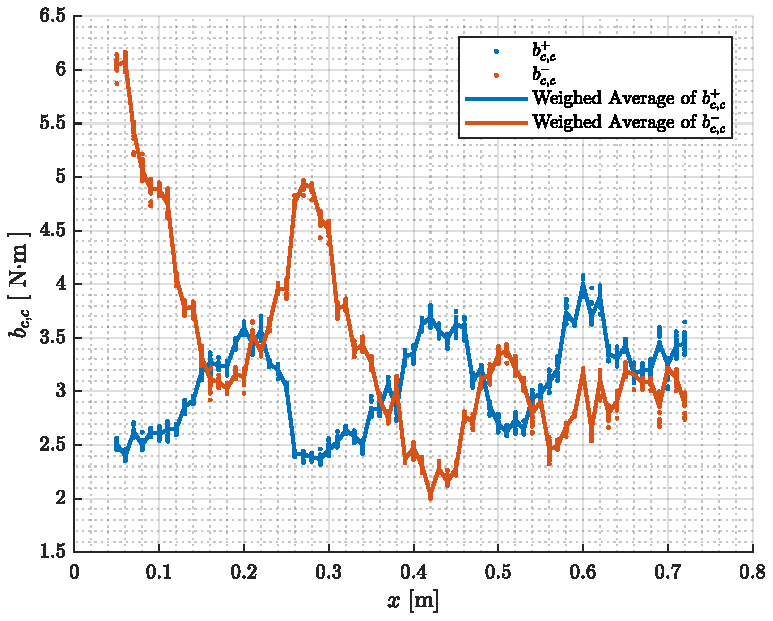
\includegraphics[width=.45\textwidth]{figures/cartColoumb}
  }
  \hspace{20pt}
  \captionbox 
  {
    cartErrn
    \label{fig:cartErrn}
  }
  {
    \hspace{-1cm}
    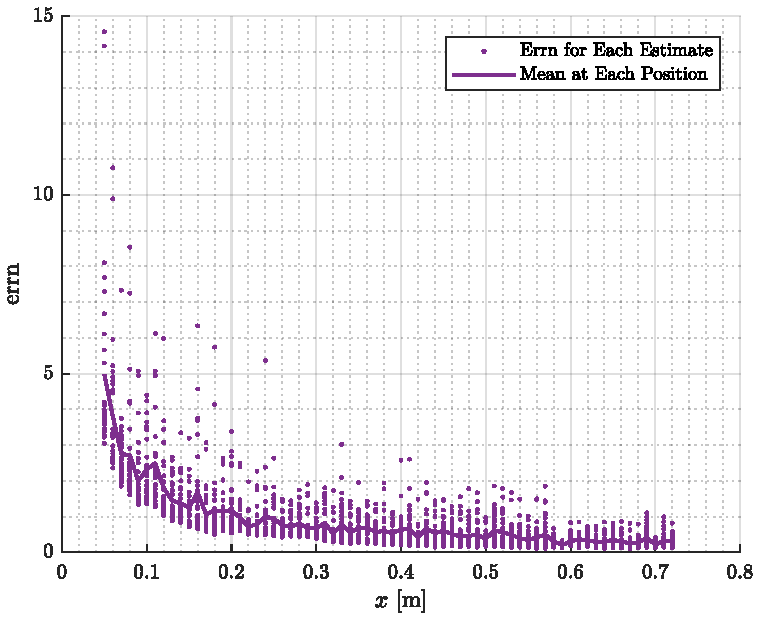
\includegraphics[width=.45\textwidth]{figures/cartErrn}
  }  
\end{figure}

\begin{figure}[H]
  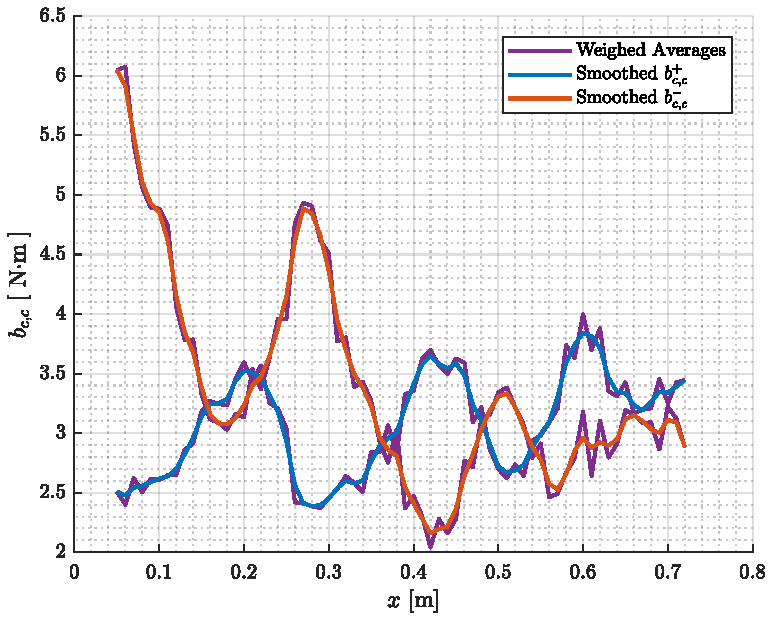
\includegraphics[width=.42\textwidth]{figures/cartColoumbSmoothDownSample}
  \caption{cartColoumbSmoothDownSample}
  \label{fig:cartColoumbSmoothDownSample}
\end{figure}


\subsection{Pendulum Friction}
\fxnote{Write about pendulum friction}

$m l ^2 \ddot{\theta} = m g l  \sin \theta - b_{p,v} \dot{\theta} - \tanh(k_{tanh} \dot{\theta}) b_{p,c} $

\section{MA Filter Design}
The measurements in the system are the position, $x$, of the cart and the angle, $\theta$, of the pendulum. Thus, the last two states, $\dot{x}$ and $\dot{\theta}$, must be estimated for the implementation. To that end, a numerical differentiation is applied to the position measurements in order to obtain the velocities,
\begin{align}
  \dot{x} &= \frac{x_0 - x_{-1}}{T_{s}}   \ \ \ ,
  \label{eq:nummericalDiff}
\end{align}
where $T_s$ is the sample time and $x_0$ and $x_{-1}$ are the two latest samples. However, this approach causes noise in the velocities. Thus, an MA (Moving Average) filter is designed to smooth the signal,
%
\begin{align}
  \dot{x}_{est} &= \frac{1}{N}\sum_{i=1-N}^{0} \dot{x}_i   \ \ \ ,
  \label{eq:MA}
\end{align}
%
where $\dot{x}_0$ is the numerical differentiation based on the two latest measurements, $x_{est}$ is the filtered value and $N$ is the window size of the filter. In \autoref{fig:thetaDotMA_design} and \ref{fig:xDotMA_design} the MA filter is applied to the result of the numerical differentiation with two different window sizes. Since the interest here is quality of the signal, the following plots are not linked in time, but rather showing the signals where the filter characteristics shows clearly.
%
\begin{figure}[H]
  \hspace{1cm}
  \captionbox
  {
    The result of applying the MA filter to the numerical differentiation of $\theta$ with two window sizes. For $N = 5$ a lot of noise is still in the signal, however, though $N=15$ removes more noise it also introduces unwanted delay. 
    \label{fig:thetaDotMA_design}
  }
  {
    \hspace{-1cm}
    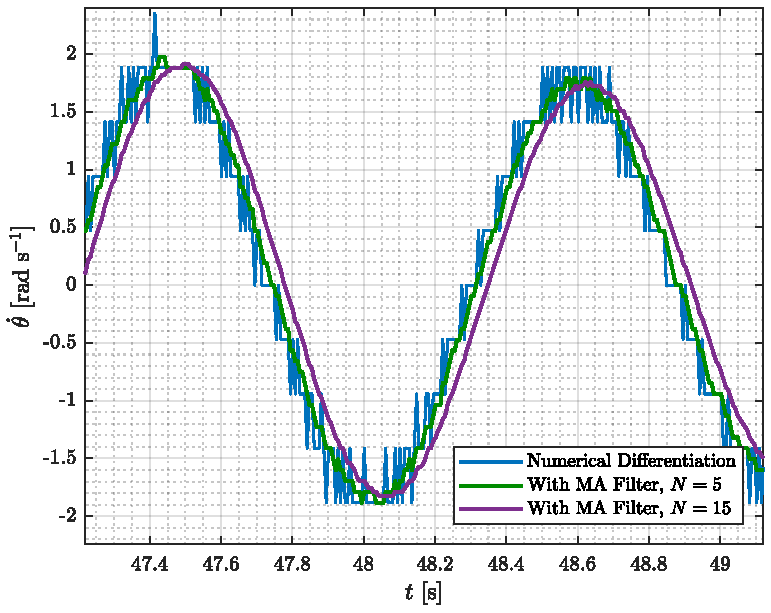
\includegraphics[width=.45\textwidth]{figures/thetaDotMA_design}
  }
  \hspace{20pt}
  \captionbox 
  {
    For $\dot{x}$ the same result is observed, but since the signal is smaller relative to the noise, it more clearly shows the noise issue of the small window size.
    \label{fig:xDotMA_design}
  }
  {
    \hspace{-1cm}
    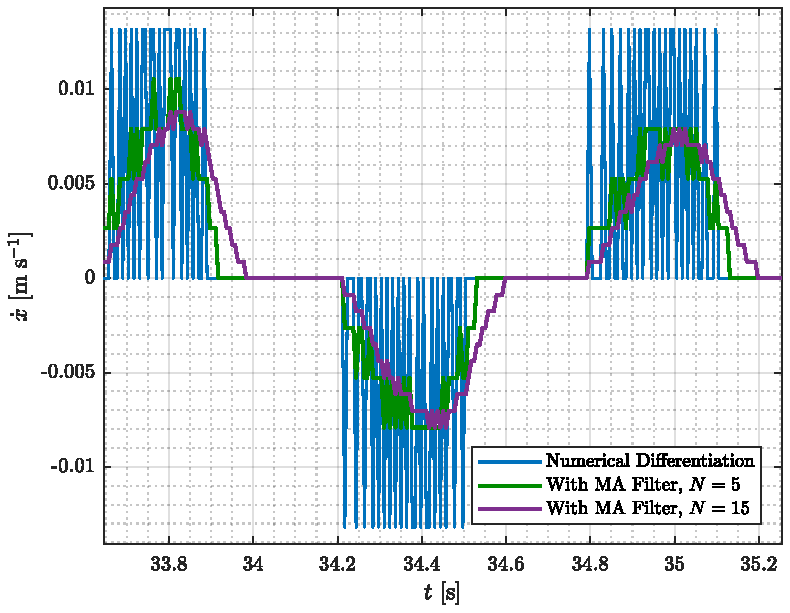
\includegraphics[width=.45\textwidth]{figures/xDotMA_design}
  }  
\end{figure}
%
The filter is implemented using a ring-buffer to minimize computation time and different window sizes are tested. Minimizing delay of the filter turns out to be more critical than further noise reduction, so a window size of five is chosen. The result of the implemented MA filter is shown in \autoref{fig:thetaDotMA_test} and \ref{fig:xDotMA_test}.
%
\begin{figure}[H]
  \hspace{1cm}
  \captionbox
  {
    The resulting implementation of the MA filter with $N=5$ for estimation of $\dot{\theta}$.
    \label{fig:thetaDotMA_test}
  }
  {
    \hspace{-1cm}
    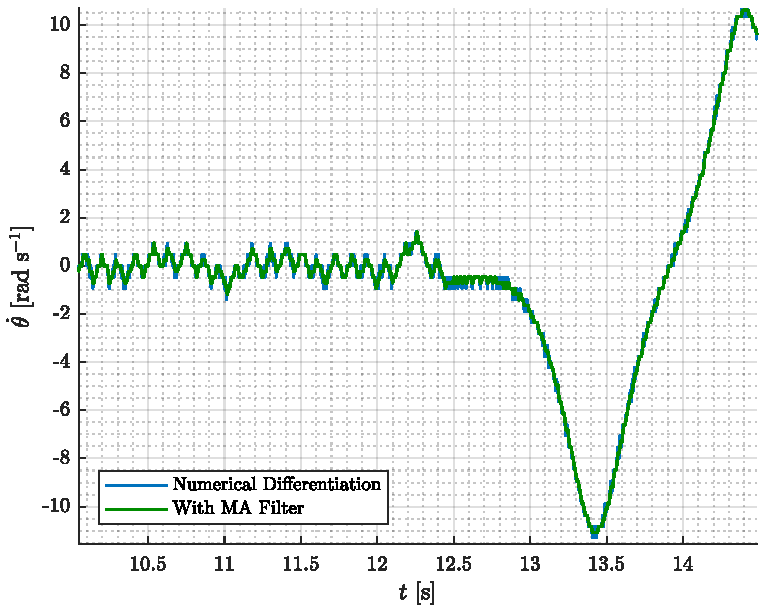
\includegraphics[width=.45\textwidth]{figures/thetaDotMA_test}
  }
  \hspace{20pt}
  \captionbox 
  {
    The implemented MA filter with $N=5$ for estimation of $\dot{x}$.
    \label{fig:xDotMA_test}
  }
  {
    \hspace{-1cm}
    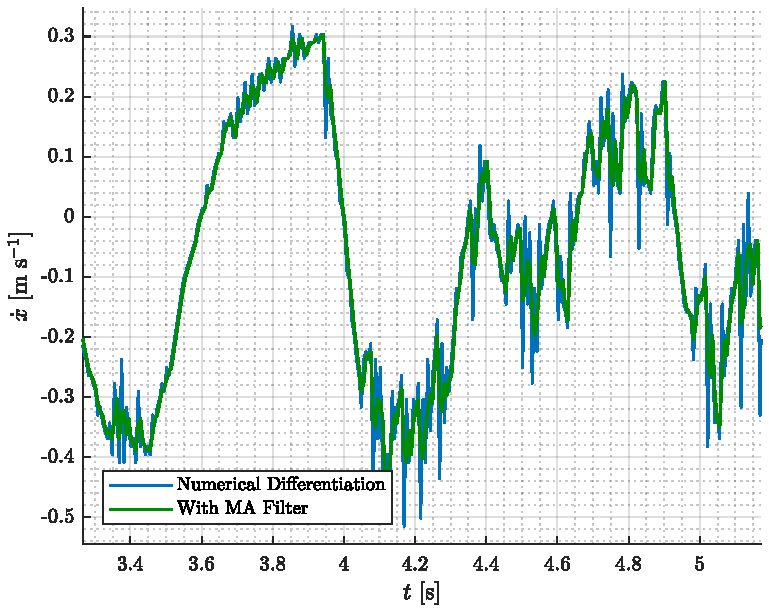
\includegraphics[width=.45\textwidth]{figures/xDotMA_test}
  }  
\end{figure}
%
Though the MA filter still lets a lot of noise through, the design does suppress large jumps in the velocity with very minimal delay.\\
This filter is only used in the swing-up sequence, an extended Kalman filter (EKF) implemented by a previous project group, \cite{JHHorgensen}, is used for the catch sequence as the switching nature of a sliding mode controller would cause oscillations with high noise levels around zero.